\documentclass[../../../main.tex]{subfiles}
\begin{document}

%%%%%%%%%%%%%%%%%%%%%%%%%%%%%%%%%%%%%%%%%
%%%%%%%%%%%%%%%%%%%%%%%%%%%%%%%%%%%%%%%%%
%%%%%%%%%%%%%%%%%%%%%%%%%%%%%%%%%%%%%%%%%
\chapter{Discrete probability distribution functions}


Recall that a function can be characterized as a mapping or assignment, or even a look up table. In essence, a function pairs every element from one set with an element from another set. That is to say, it assigns to each value in one set a value from another set.

A probability distribution function (\PDFtext/ for short) is a function that assigns a probability to each possible outcome of an experiment. So it is a lookup table for the probability of all outcomes.

To build a \PDFtext/, we make a table. In one column, we put down all the values an experiment can have. In another column, we put down the probability of that outcome. 

\paragraph{Notation reminder:}

The value of a random variable is symbolized as a lower case letter, like $\RandVarVal/$. The probability of a value $\RandVarVal/$ is written $\Probability{\RandVarVal/}$. So when we build a \PDFtext/, we essentially calculate $\Probability{\RandVarVal/}$ for each $\RandVarVal/$ of an experiment, and we put that all down in a table.

Every \PDFtext/ function has two important characteristics.

\begin{itemize}

  \item Every $\Probability{\RandVarVal/}$ must be between 0 and 1. This should not be a surprise. Every probability falls between 0 and 1, since a probability is just the percentage chance that something will happen, which in statistics we typically speak about a percentage as the fraction or decimal between 0 and 1.

  \item If we sum up $\Probability{\RandVarVal/}$ for each $\RandVarVal/$, the probabilities must all add up to 1. This should also make sense. If there's a 50\% (.5) chance that I can flip a heads, then the chance of getting tails must be the remainder of the chances, namely the other 50\% (the other .5). If there are two red marbles and a blue marble in a bag, the chances of getting a red is 2 out of 3, and the other 1 out of 3 is for the blue marble. There's always a total of 1 (100\%) for all the options, taken together.

\end{itemize}

A \PDFtext/ shows us where the probabilities are distributed. Since there can only be a total of 1 (100\%), how is that broken up? How much of that gets divided up across the different possible outcomes?

A \PDFtext/ identifies exactly how much of the total probability is assigned to each outcome. If we plot it (with a bar plot), we can even see plotically how much of the probability is distributed to each outcome.


%%%%%%%%%%%%%%%%%%%%%%%%%%%%%%%%%%%%%%%%%
%%%%%%%%%%%%%%%%%%%%%%%%%%%%%%%%%%%%%%%%%
\section{Example 1}

Let the experiment be flipping a fair coin. So, the random variable $\RandVar/$ is:

\begin{equation*}
    \RandVar/ = \text{ the outcome of flipping a fair coin}
\end{equation*}

\noindent
And the values are:

\begin{equation*}
    \RandVarVal/ = \{ H, T \} \hskip 1cm \text{ or } \hskip 1cm \{ 1, 0 \}
\end{equation*}

\noindent
What are the probabilities of each outcome? Well, the probability of heads is 0.5, and the probability of tails is 0.5. Each outcome has a 50\% chance of happening.

Let's make a table that maps the outcomes to the probabilities:

\begin{center}
  \begin{tabular}{| c | c |}
    \hline
    $\RandVarVal/$ & $\Probability{\RandVarVal/}$ \\ \hline
               H & 0.5 \\ \hline
               T & 0.5 \\ \hline
  \end{tabular}
\end{center}

\noindent
If you like, we can draw this as a map:

\begin{center}\begin{tikzpicture}

  \node[] (H) [] {$H$};
  \node[] (T) [below=of H] {$T$};
  \node[] (a) [right=6cm of H] {$0.5$};

  \path[->] (H) edge (a);
  \path[->] (T) edge (a);

\end{tikzpicture}\end{center}

\noindent
Or, we can write it out as a set of pairs:

\begin{equation*}
    \Pdf{\RandVarVal/} = \{ (H, 0.5), (T, 0.5) \}
\end{equation*}

\noindent
Then we can use this to lookup the probability for a particular outcome. Remember the notation $f(x) = y$, which we read as ``$f$ maps $x$ to $y$,'' or ``the value that $f$ pairs up with $x$ is $y$,'' or ``lookup $x$ in the $f$ lookup table, and you get $y$.'' 

In our example, we can use this notation. What is the probability of getting heads? That is, what is $\Pdf{\RandVarVal/ = H}$ or $\Pdf{H}$? It is this:

\begin{equation*}
    \Pdf{H} = 0.5
\end{equation*}

\noindent
Read that like this: ``$\Pdf{\RandVarVal/}$ maps $H$ to 0.5,'' or ``the value that $\Pdf{\RandVarVal/}$ pairs up with $H$ is 0.5,'' or ``lookup $H$ with the $\Pdf{\RandVarVal/}$ lookup table, and you get 0.5.''

And what is the probability of getting tails? That is, what is $\Pdf{\RandVarVal/ = T}$ or $\Pdf{T}$? It is this:

\begin{equation*}
    \Pdf{T} = 0.5
\end{equation*}

\noindent
Let's plot it. See Figure \ref{plot:example-1}.

\begin{figure}[ht]
  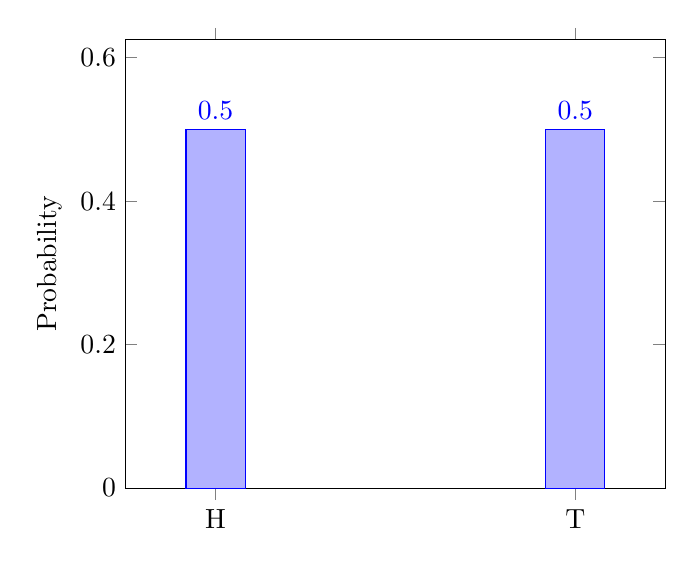
\begin{tikzpicture}
    \centering
    \begin{axis} [
      ylabel=Probability,
      symbolic x coords={H, T},
      ybar,
      xtick=data,
      ymin=0,
      enlarge y limits={value=0.25,upper},
      enlarge x limits=0.25,
      nodes near coords,
      bar width=0.75cm,
      ]
      \addplot coordinates {(H, 0.5) (T, 0.5)};
    \end{axis}
  \end{tikzpicture}
  \caption{\label{plot:example-1} $\Probability{\RandVarVal/}$ for coin flip}
\end{figure}

So, how are the probabilities distributed in this experiment? They are distributed evenly. Each outcome gets half of the total. 

We say that this is a \vocab{uniform} probability distribution. We call it ``uniform'' because the probabilities are distributed evenly.


%%%%%%%%%%%%%%%%%%%%%%%%%%%%%%%%%%%%%%%%%
%%%%%%%%%%%%%%%%%%%%%%%%%%%%%%%%%%%%%%%%%
\section{Example 2}

Let the experiment be rolling a fair six-sided die. The outcome of rolling a die is a \emph{discrete random variable}:

\begin{equation*}
    \RandVar/ = \text{ the outcome of rolling a fair six-sided die}
\end{equation*}

\noindent
Its values are:

\begin{equation*}
    \RandVarVal/ = \{ 1, 2, 3, 4, 5, 6 \}
\end{equation*}

\noindent
What are the probabilities of these outcomes? For each it is one out of six, or $\frac{1}{6}$, or 0.167.

Let's make a table that maps the outcomes to the probabilities:

\begin{center}
  \begin{tabular}{| c | c |}
    \hline
  $\RandVarVal/$ & $\Probability{\RandVarVal/}$  \\ \hline
               1 & 0.167 \\ \hline
               2 & 0.167 \\ \hline
               3 & 0.167 \\ \hline
               4 & 0.167 \\ \hline
               5 & 0.167 \\ \hline
               6 & 0.167 \\ \hline
  \end{tabular}
\end{center}

\noindent
We can draw this function as a map:

\begin{center}\begin{tikzpicture}

  \node[] (1) [] {$1$};
  \node[] (2) [below=of 1] {$2$};
  \node[] (3) [below=of 2] {$3$};
  \node[] (4) [below=of 3] {$4$};
  \node[] (5) [below=of 4] {$5$};
  \node[] (6) [below=of 5] {$6$};
  \node[] (a) [right=6cm of 1] {$0.167$};

  \path[->] (1) edge (a);
  \path[->] (2) edge (a);
  \path[->] (3) edge (a);
  \path[->] (4) edge (a);
  \path[->] (5) edge (a);
  \path[->] (6) edge (a);

\end{tikzpicture}\end{center}

\noindent
Or, we can write it out as a set of pairs:

\begin{equation*}
    \Pdf{\RandVarVal/} = \{ (1, 0.167), (2, 0.167), (3, 0.167), (4, 0.167), (3, 0.167), (6, 0.167) \}
\end{equation*}

\noindent
We can lookup particular values if we like. What is the probability of rolling a 4? That is, what is $\Pdf{\RandVarVal/ = 4}$ or $\Pdf{4}$?

\begin{equation*}
    \Pdf{4} = 0.167
\end{equation*}

\noindent
Let's plot it. See Figure \ref{plot:example-2}.

\begin{figure}[ht]
  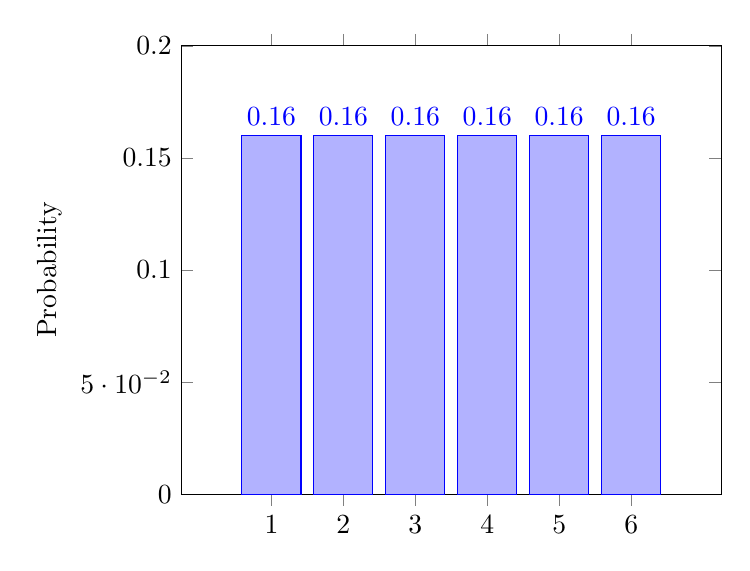
\begin{tikzpicture}
    \centering
    \begin{axis} [
      ylabel=Probability,
      symbolic x coords={1, 2, 3, 4, 5, 6},
      ybar,
      xtick=data,
      ymin=0,
      enlarge y limits={value=0.25,upper},
      enlarge x limits=0.25,
      nodes near coords,
      bar width=0.75cm,
      ]
      \addplot coordinates {(1, 0.16) (2, 0.16) (3, 0.16) (4, 0.16) (5, 0.16) (6, 0.16)};
    \end{axis}
  \end{tikzpicture}
  \caption{\label{plot:example-2} $\Probability{\RandVarVal/}$ for dice roll}
\end{figure}

So, how are the probabilities distributed in this experiment? If we look in the plot, we can see that they are distributed evenly. Each outcome gets one-sixth of the total. So this is also a \vocab{uniform} distribution.



%%%%%%%%%%%%%%%%%%%%%%%%%%%%%%%%%%%%%%%%%
%%%%%%%%%%%%%%%%%%%%%%%%%%%%%%%%%%%%%%%%%
\section{Example 3}

Suppose we have a bag with 5 marbles in it. Three are red, one is blue, and one is green.
Let the experiment be that we reach into the bag blindfolded, and we pull out one marble.

The outcome of drawing a marble from the bag is a \emph{discrete random variable}:

\begin{equation*}
    \RandVar/ = \text{ the outcome of blindly drawing a marble from the bag }
\end{equation*}

\noindent
We could say that the values are ``$red_{1}$,'' ``$red_{2}$,'' ``$red_{3}$,'' ``$blue$,'' and ``$green$'' (or, if we want to use numbers, we could say ``1,'' ``2,'' ``3,'' ``4,'' and ``5'' respectively). But let's group the colors together and say that the outcome we are interesting in is whether one gets a red, blue, or green marble, which we'll notate as ``$R$,'' ``$B$,'' or ``$G$'' (or ``1,'' ``2,'' ``3,'' if you want numbers):

\begin{equation*}
    \RandVarVal/ = \{ R, B, G \} \hskip 1cm \text{ or } \hskip 1cm \{ 1, 2, 3 \}
\end{equation*}

\noindent
What are the probabilities of these outcomes? The probability of getting $R$ (a red) is 3 out of 5, or $\frac{3}{5}$, or 0.6. The probability of getting $B$ (a blue) is 1 out of 5, or 0.2, and likewise for getting $G$ (a green). 

Let's make a table that maps the outcomes to the probabilities:

\begin{center}
  \begin{tabular}{| c | c |}
    \hline
  $\RandVarVal/$ & $\Probability{\RandVarVal/}$ \\ \hline
               R & 0.6 \\ \hline
               B & 0.2 \\ \hline
               G & 0.2 \\ \hline
  \end{tabular}
\end{center}

\noindent
We can draw this function as a map:

\begin{center}\begin{tikzpicture}

  \node[] (R) [] {$R$};
  \node[] (B) [below=of R] {$B$};
  \node[] (G) [below=of B] {$G$};
  \node[] (a) [right=6cm of R] {$0.6$};
  \node[] (b) [right=6cm of B] {$0.2$};

  \path[->] (R) edge (a);
  \path[->] (B) edge (b);
  \path[->] (G) edge (b);

\end{tikzpicture}\end{center}

\noindent
Or, we can write it out as a set of pairs:

\begin{equation*}
    \Pdf{\RandVarVal/} = \{ (R, 0.6), (B, 0.2), (G, 0.2) \}
\end{equation*}

\noindent
We can lookup particular values if we like. What is the probability of pulling out a red marble? That is, what is $\Pdf{\RandVarVal/ = R}$ or $\Pdf{R}$?

\begin{equation*}
    \Pdf{R} = 0.6
\end{equation*}

\noindent
And what is the probability of pulling out a green marble?

\begin{equation*}
    \Pdf{G} = 0.2
\end{equation*}

\noindent
Let's plot it. See Figure \ref{plot:example-3}.

\begin{figure}[ht]
  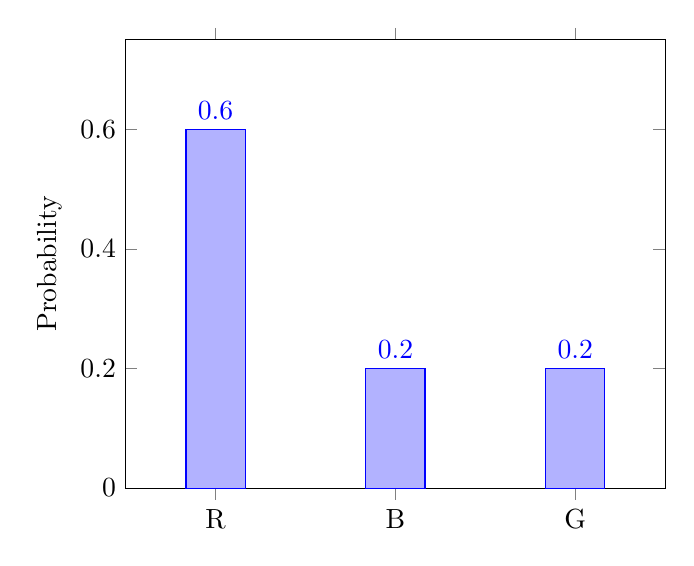
\begin{tikzpicture}
    \centering
    \begin{axis} [
      ylabel=Probability,
      symbolic x coords={R, B, G},
      ybar,
      xtick=data,
      ymin=0,
      enlarge y limits={value=0.25,upper},
      enlarge x limits=0.25,
      nodes near coords,
      bar width=0.75cm,
      ]
      \addplot coordinates {(R, 0.6) (B, 0.2) (G, 0.2)};
    \end{axis}
  \end{tikzpicture}
  \caption{\label{plot:example-3} $\Probability{\RandVarVal/}$ for drawing one marble}
\end{figure}

Where are the probabilities distributed? In the plot, we can see that most of the probability falls on red. This makes sense, of course, since there are more red marbles in the bag than green or blue. But this visually lets us see exactly where the probability gets chunked up (distributed). Note that this is not a uniform distribution.


%%%%%%%%%%%%%%%%%%%%%%%%%%%%%%%%%%%%%%%%%
%%%%%%%%%%%%%%%%%%%%%%%%%%%%%%%%%%%%%%%%%
\section{Other kinds of distributions}

We have looked at just a few very simple \PDFtext/s, in order to help us get a feel for what exactly a \PDFtext/ is. There are a number of very specialized \PDFtext/s, which are very useful in statistics. We turn to some of these next.



\end{document}
